\documentclass[a4paper,11pt]{article}

\usepackage{graphicx}
\usepackage[printwatermark]{xwatermark}
\usepackage[margin=1in]{geometry}
\usepackage[doublespacing]{setspace}
\usepackage{color} % needed if you use xfig graphics at all
\usepackage{xcolor}
\usepackage{url}
\usepackage{hyperref}
\usepackage{csquotes}
\usepackage{listings}
\usepackage{courier}
\usepackage{subfigure}
\usepackage{mdwlist}
\usepackage{tabu}
\usepackage{array,etoolbox}
\usepackage{lscape}
\usepackage{rotating}
\usepackage[toc,page]{appendix}
\usepackage{pdfpages}
\usepackage{pdflscape}	%allows landscape orientation for floats
\usepackage{afterpage}
\usepackage{ragged2e}
\usepackage{textcomp}
\usepackage{mdwlist}
\usepackage{amsmath}	% allows \text{} in math mode $$ or \[ \]
\usepackage{amsthm}		%used for defining theorems
\usepackage{longtable} % for 'longtable' environment



%\subtitle{File System Forensics Masterclass}
\author{Fraser Brown}
%\institute{Heriot-Watt University}
\date{\today}

\graphicspath{{../figures/}}

\begin{document}

%Title
\begin{titlepage}
   \vspace*{\stretch{1.0}}
   \begin{center}
      \Large\textbf{Digital Forensics Masterclass Labsheet}\\
      \large\textit{File System Forensics}
   \end{center}
   \vspace*{\stretch{2.0}}
\end{titlepage}

\tableofcontents
\newpage

\section{Lab Overview}
The learning objective for this lab is for participants to gain practical experience in digital forensics specifically file system analysis. During the lab you will gain experience in the following tools, environments and tasks:
\begin{itemize*}
	\item Kali Linux\footnote{https://www.kali.org/}
	\item The Sleuth Kit (TSK)\footnote{https://www.sleuthkit.org/} file system analysis tool kit.
	\item Forensic image creation.
	\item Identifying Attributes about file systems (data uni size file type).
	\item Deleted file recover procedure.
	\item Searching for evidence on a file system.
	\item Event timeline creation?????
\end{itemize*}

As an \textit{optional} bit of fun for the lab, we will be adding a capture the flag (CTF) style element. For each task there is a set goal, that may be finding a word or phrase in unallocated space, the hash of a recovered file etc. After each task is completed please enter the given evidence as an argument to the \texttt{flagfound} script as follows:\\
\verb|$  ./flagfound "YOUR EVIDENCE HERE"|


\section{Removable Media Resource Credits}
The USB resources we will be using in today's lab are from the National Institute of Standards and Technology (NIST) as part of their Computer Forensic Reference Data Sets (CFReDS)\footnote{https://www.cfreds.nist.gov/}.  We will be focusing on a subsection of this case using ``Removable Media {\#}2'', in order to investigate material covered in the lecture. The scenario section below will set the scene. 
 
 If you are interested in exploring this scenario more the whole case can be fond here:\\
 \verb|https://www.cfreds.nist.gov/data_leakage_case/data-leakage-case.html|

\section{Environment Setup}
\subsection*{Installing Kali Linux in Virtual Box}
Before your digital investigation can begin you are required to create a lab environment, for this we will be using a virtual machine (VM) instance of Kali Linux.
Your user accounts should have been given access to virtual box in the university lab (EM2.50). We are using a virtual machine to no only give you complete control over the operating system, but so this lab can be carried out safely. Below we will show you how to create a Kali Linux VM.
	\begin{enumerate*}
	 \item Open a terminal window and enter the following command to open Virtual Box:\\
		\texttt{{\$}	virtualbox {\&}}
	\item Return to the terminal window and follow \texttt{LoadingKaliVM.pdf} instructions, created by Mike Just.
	\item Start your Kali VM
	\end{enumerate*}
	
\subsection{Kali Login Information}
\begin{itemize*}
	\item username: \texttt{root}
	\item password: \texttt{toor}
\end{itemize*}

\subsection{Note About Root}
In Kali Linux you are logged in as the root user of the system, therefore the operating system assumes you know what you are doing. Double check the commands you are entering especially if they are related to \texttt{rm}.

\subsection{Create a Case Directory for Investigation}
Within your home directory create the a \texttt{cases} directory and inside that create a directory called \texttt{001} to represent the case number you are working on. Make this your current working directory in a terminal window.

\newpage
\section{Task 1: Create a Forensic Image}
There should be USB flash drives available for this lab, with the removable media evidence on them.  In this lab we will be working with .dd images also known as raw images. There are many tools available to create the a forensic image with Kali Linux comes installed with both GUI and command line versions. It is up to you which you use however I would recommend \texttt{Guymager}.\\

\textbf{NOTE:} \textit{Sadly we were not able to attain writeblockers for this lab, please remember that writeblockers are important for prevention of unwanted meta data changes to media by the investigators operating system. Writeblockers are used in industry when creating forensic images of a system.}\\

Insert USB Stick into computer and confirm it has been recognised by the Kali Linux VM, you can check this in either in files that a usb device is visable in the left hand pane or by running \texttt{df -h} in the command line and checking for a 4GB device located in \texttt{/media/root/}. \\

Open a terminal window (we will use this later anyway) and enter: \texttt{guymager {\&}} the following GUI should appear:
\begin{figure}[h]
	\centering
	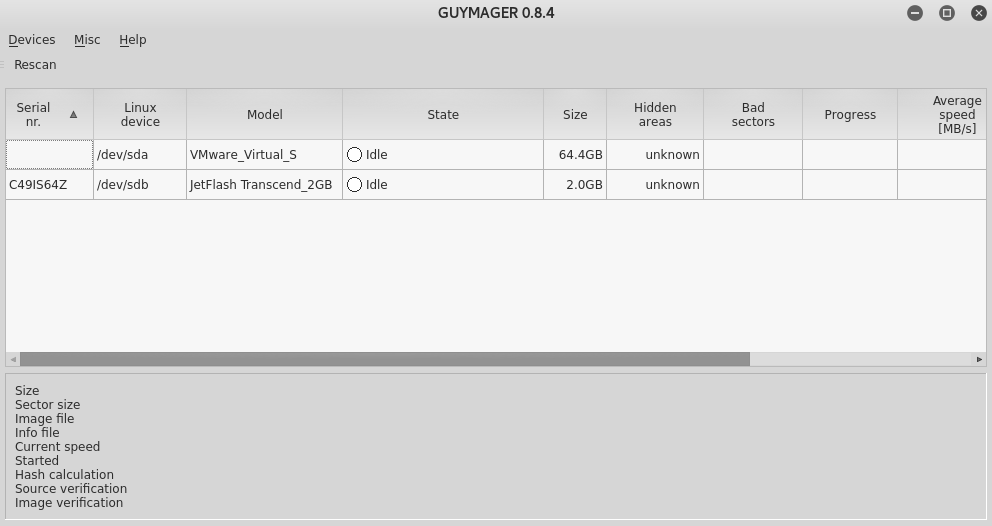
\includegraphics[scale=0.5]{guymager-window}
	\caption{\textit{guymager gui window example}}
	\label{fig:guymager-main-window}
\end{figure}
\\
If the 4GB usb drive does not show up press \texttt{f5} to rescan devices. From here you can select the drive you wish to create an image of, right click the 4GB drive and select the \texttt{Aquire image} option. Fill out the guy form making sure you have the following options then click start:
\begin{itemize*}
\item Linux dd raw image
\item Uncheck split image
\item Destination is set to \texttt{/home/cases/001/image/}
\item Image filename set to \texttt{revmed2}
\item Info filename set to \texttt{revmed2}
\item Check calculate md5 hash
\item Check verify image after acquisition
\end{itemize*}
\begin{figure}
	\centering
	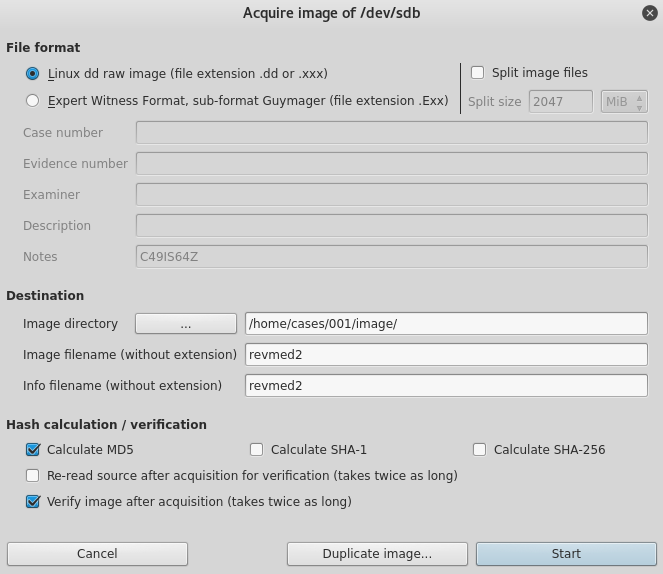
\includegraphics[scale=0.5]{guymager-aquisition-window}
	\caption{\textit{guymager acquisition window example}}
	\label{fig:guymager-aquisition-window}
\end{figure}

Once you have clicked start you shall be returned to the main guymager window and a progress bar should be displayed. once the progress bar states ``Finished - Verified {\&} ok'' your forensic image has been created. To confirm list the contents of \texttt{/home/cases/001/image/} in a terminal window, you should find the following files: 
\begin{itemize*}
\item \texttt{revmed2.dd} : the image file we can now perform analysis on.
\item \texttt{revmed2.info} : acquisition info such as cryptographic hash.
\end{itemize*}

\subsubsection*{Verify The Media Hash}
in order to confirm that our image is the same as the contents of the USB we must generate a hash of the .dd file and compare it to the hash listed in the .info file.
in a terminal window run the following:
\texttt{md5sum image/revmed2.dd}
the output should match the hash listed in the .info file you just created.

Remove the USB from your machine and return it to the evidence box.

\textit{\textbf{Optional:} enter the hash into the \texttt{findflag} program to receive your first flag.}

\section{Task 2: File System Identification}
Now that we have a forensic image we can start to analyse the evidence.


\section{Task 3: Deleted File Recovery}

\section{Task 4: Searching Unallocated Space for Evidence}



\end{document}